\documentclass[smaller, dvipsnames]{beamer}

\usetheme[numbering=fraction,%
          block=fill,%
          sectionpage=progressbar,%
          subsectionpage=progressbar,%
]{metropolis} % Use metropolis theme
\setbeamercovered{invisible}

\usepackage[utf8]{inputenc}
\usepackage[T1]{fontenc}

\usepackage{xspace}
\usepackage{booktabs}
\usepackage{amssymb}
\usepackage{tikz}
\usetikzlibrary{arrows} % required in the preamble
\usepackage{smartdiagram}
\usesmartdiagramlibrary{additions} % required in the preamble

\newcommand{\ah}{Angry-HEX\xspace}
\newcommand{\ab}{Angry Birds\xspace}
\newcommand{\abc}{Angry Birds AI Competition\xspace}
\newcommand{\al}{Alpha\xspace}

\title{Complex Predicates vs.\ Complex Objects}
\subtitle{A Case Study on ASP for Implementing Artificial Agents}
\author{Filippo De Bortoli \and Lorenz Leutgeb \and Cosimo Persia}
\institute{European Master's Program in Computational Logic, TU Dresden}
\date{February 16th, 2018}

\begin{document}

\maketitle

\begin{frame}{Outline}
    \tableofcontents
\end{frame}

\section{Introduction}

\subsection{Angry Birds}

\begin{frame}{The Game}
	\begin{figure}
  		
\includegraphics[width=300pt]{./img/angry-birds.jpg}
	\end{figure}
	\begin{itemize}
		\item<1-> Eliminate all pigs
		\item<2-> Reach high score
	\end{itemize}
\end{frame}

\begin{frame}{Challenges for AI}
	 \begin{columns}
		 \begin{column}{0.5\textwidth}
			\begin{itemize}
				\item<1->[] Physics
				{\par\centering\includegraphics<1>[width=4.5cm]{./img/birds-square}\par}
				\item<2->[] Planning
				{\par\centering\includegraphics<2>[width=4.5cm]{./img/planning.png}\par}
			\end{itemize}
		 \end{column}
		 \begin{column}{0.5\textwidth}
			\begin{itemize}
			\item<3->[] Computer Vision
    		{\par\centering\includegraphics<3>[width=4.5cm]{./img/object-detection}\par}
    		\item<4->[] Knowledge Representation
  		\end{itemize}
		 \end{column}
	 \end{columns}
\end{frame}

\begin{frame}{Our Motivation}
	\begin{itemize}
		\item Find an existing, interesting agent based on logic programming (ASP). Angry-HEX
		\item Understand how it works.
		\item Figure out how to adapt it to the Alpha system.
		\item Structure and formalize the learnings.
		\item Improve over the agent!
	\end{itemize}
\end{frame}

\subsection{ASP and HEX-programs}

\begin{frame}{Declarative Programming}
 	\begin{center}
 	\begin{itemize}
	\item<1->[] ALGORITHM = LOGIC + CONTROL
		\begin{align*}
			&append ([\:], X, X). \\
			&append ([X|Y], Z, [X|T ]) \leftarrow append (Y, Z, T ). \\
			&reverse([ ], [ ]).\\
			&reverse([X|Y ], Z) \leftarrow append (U, [X], Z), reverse(Y, U ).
		\end{align*}
  \item<2>[] Order of clauses and subgoals does not matter.
  		\begin{align*}
			reverse([X|Y], Z) \leftarrow reverse(Y, U ), append (U, [X], Z).
		\end{align*}
	\end{itemize}	
	\end{center}
 
\end{frame}

\begin{frame}{Stable Model Semantics}
    \begin{center}
    	\begin{align*}
			&pig((88,34)). \\
			&easy\_target(X) \leftarrow pig(X), not\: difficult\_target(X). \\ 
			&difficult\_target(X) \leftarrow pig(X), not\: easy\_target(X). 
		\end{align*}
    \end{center}
    \begin{itemize}
    	\item<2->[] models which reflects natural intuition
    	\item<3->[]
    		\begin{align*}
				&\only<4>{\textcolor{red}}{ M_1= \{pig((88,34)), easy\_target((88,34))\}  } \\
				&\only<4>{\textcolor{red}}{ M_2= \{pig((88,34)), difficult\_target((88,34))\}  }\\
				&M_3= \{pig((88,34)), easy\_target((88,34)), difficult\_target((88,34))\}
    		\end{align*}
    \end{itemize}
\end{frame}
%maybe another example of stable model here

\begin{frame}{External Atoms}
    \begin{itemize}
    	\item<1-> They allow bidirectional communication with external sources
    	\item<2->[] \[ \&g[q_1,\dots,q_k](t_1,\dots,t_l) \]
    	\item<3-> Example: we want to use an arbitrary computable function that access an rdf file from the web
    	\item<4->[] \[ \&rdf[url](X,Y,Z) \]
    	\item<5->[] 
    		\begin{align*}
				bel(X,Y,Z) \leftarrow \&rdf[url](X,Y,Z)
    		\end{align*}
    \end{itemize}
\end{frame}

\begin{frame}{HEX-programs}
    \begin{itemize}
    	\item<1-> Generalization of disjunctive extended logic programs under the answer set semantics.
    	\item<2-> Rules
    	\item<2->[] \[ a_1, \lor \dots \lor a_n \leftarrow b_1, \dots , b_m, \neg b_{m+1}, \dots, b_n \; (m,n \geq 0)\]
    	\item<3-> External atoms
    	\item<3->[] \[ \&g[q_1,\dots,q_k](t_1,\dots,t_l) \]
    \end{itemize}
\end{frame}

\section{\ah}

\begin{frame}{\ah Architecture}
	\begin{center}
		\begin{figure}
			\begin{tikzpicture}
				\node[anchor=south west,inner sep=0] at (0,0) {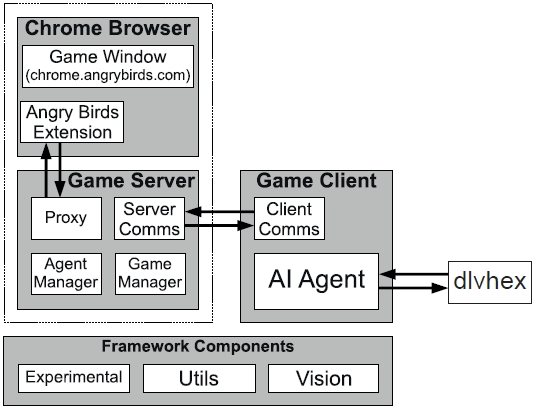
\includegraphics[scale=0.6]{./img/angryhex-agent}};
				\begin{invisibleenv}<-1>
					\draw[red,ultra thick,rounded corners] (7.1,1.6) -- (8.5,2.4);
					\draw[red,ultra thick,rounded corners] (7.1,2.4) -- (8.5,1.6);
					\node[text=red] at (7.8,2.8) {Alpha ASP};	
				\end{invisibleenv}
			\end{tikzpicture}
			\caption{Agent architecture, from \emph{Angry-HEX: An Artificial Player for Angry Birds Based on Declarative
			Knowledge Bases}, Calimeri et al., 2016}
		\end{figure}
	\end{center}
\end{frame}

\begin{frame}{Interaction with HEX-programs}
	\begin{center}
		\smartdiagramset{
%uniform color list=orange!60!yellow for 5 items,
circular final arrow disabled=false,
circular distance=2.25cm,
arrow tip=to,
arrow line width=2pt,
additions={
%additional item bottom color=orange!60!yellow,
%additional item border color=gray,
%additional item shadow=drop shadow,
additional item offset=0.65cm,
additional arrow line width=2pt,
additional arrow tip=to,
additional arrow color=orange!60!yellow,
}
}
\smartdiagramadd[circular diagram]{
Answer Set,Game Action,Game Level,Facts $\mathcal{S}$,$\mathcal{P}_{AI} \cup \mathcal{S}$
}{
left of module3/%,right of module5/End
}
\smartdiagramconnect{to-}{module3/additional-module1}
%\smartdiagramconnect{-to}{module5/additional-module2}
	\end{center}
\end{frame}

\begin{frame}
	\frametitle{DLV-HEX vs \al}
	\begin{center}
		\begin{tabular}{lcc}
			\toprule
			& DLV-HEX & \al \\
			\midrule
			Constant terms & \checkmark & \checkmark \\
			Natural numbers & \checkmark & \checkmark \\
			Strings & \checkmark & \checkmark \\
			HEX-programs & \checkmark & \\
			Java objs. interpretation & & \checkmark \\
			\bottomrule
		\end{tabular}
	\end{center}
	How to convert external and higher-order atoms to first-order atoms, using Java objects as interpretation for terms?
\end{frame}

\section{From Complex Predicates to Complex Objects}

\begin{frame}{Encoding Sets using Complex Predicates}
	A set \(s = \{ a, b, c \}\):
    \begin{align*}
    	s(a). s(b). s(c) \\
    \end{align*}

	Quantify over \(s\):
	\begin{align*}
		r(q,s).
		Z(X) \leftarrow r(Z,Y), Y(X).
	\end{align*}
\end{frame}

\begin{frame}{Encoding Sets using Complex Objects}
	A set \(s = \{ a, b, c \}\):
    \begin{align*}
    	s(\{a, b, c\}).
    \end{align*}

	Quantify over \(s\):
	\begin{align*}
		q(X) \leftarrow s(X).
	\end{align*}
\end{frame}

\begin{frame}
	\frametitle{Complexity}
\end{frame}

\begin{frame}[standout]
    Thank you!
\end{frame}

\end{document}